\documentclass{beamer}
\usepackage[utf8]{inputenc}
\usepackage{polski}
\usepackage[polish]{babel}
\usepackage[T1]{fontenc}
\usepackage{tikz}
\usepackage{tikzducks}
\usepackage{multimedia}
\usepackage{graphicx}
\usepackage{graphbox}
\usepackage[justification=centering]{caption}
\usepackage{textcomp}
\usepackage{appendixnumberbeamer}
\usepackage[width=\textwidth]{animate}

\usetheme{Warsaw}
\usecolortheme{whale}

\AtBeginSection[]{
  \begin{frame}
  \vfill
  \centering
  \begin{beamercolorbox}[sep=8pt,center,shadow=true,rounded=true]{title}
    \usebeamerfont{title}\insertsection\par%
  \end{beamercolorbox}
  \vfill
  \end{frame}
}

\title{Sky falling on our heads}
\subtitle{Analysis of material coming from the above}
\author[M. Winiarski]{Mateusz Winiarski}
\institute[Koło SIMP]{Jagiellonian University\\Faculty of Physics, Astronomy and Applied Computer Science}
\date[Szkoła Jesienna 2022]{November 24th, 2022}
%\titlegraphics{
\includegraphics[]{asterix_v4_sky_falling.jpg}}

\begin{document}

\frame{\titlepage}

\section[Part I. Observation]{Part I\\Observation: Chemtrails}

\begin{frame}
\begin{columns}[t]
\column{.5\textwidth}\vbox to \textheight{
\centering
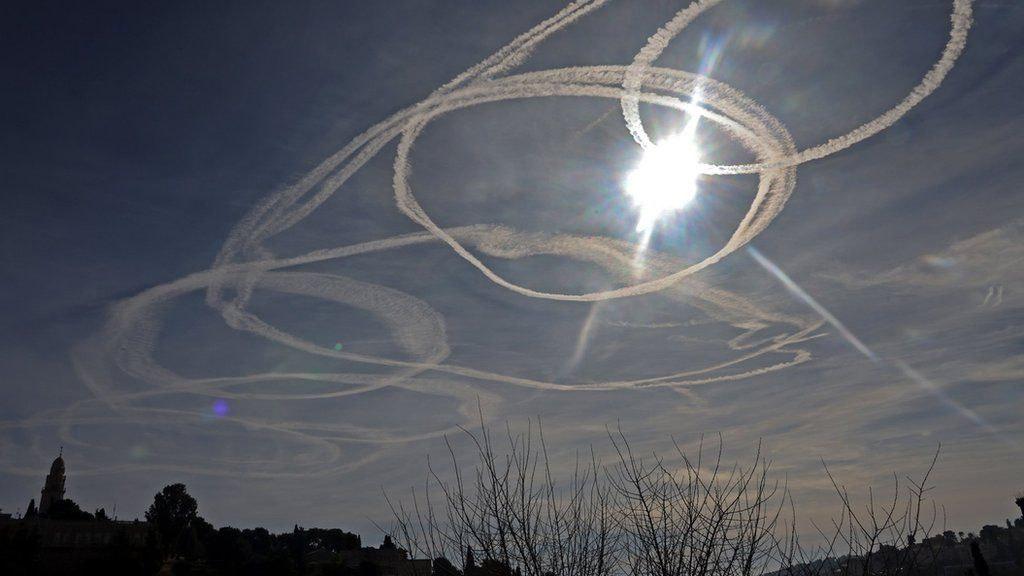
\includegraphics[width=5cm]{_126014953_gettyimages-1230798088.jpg} \\ \vfill
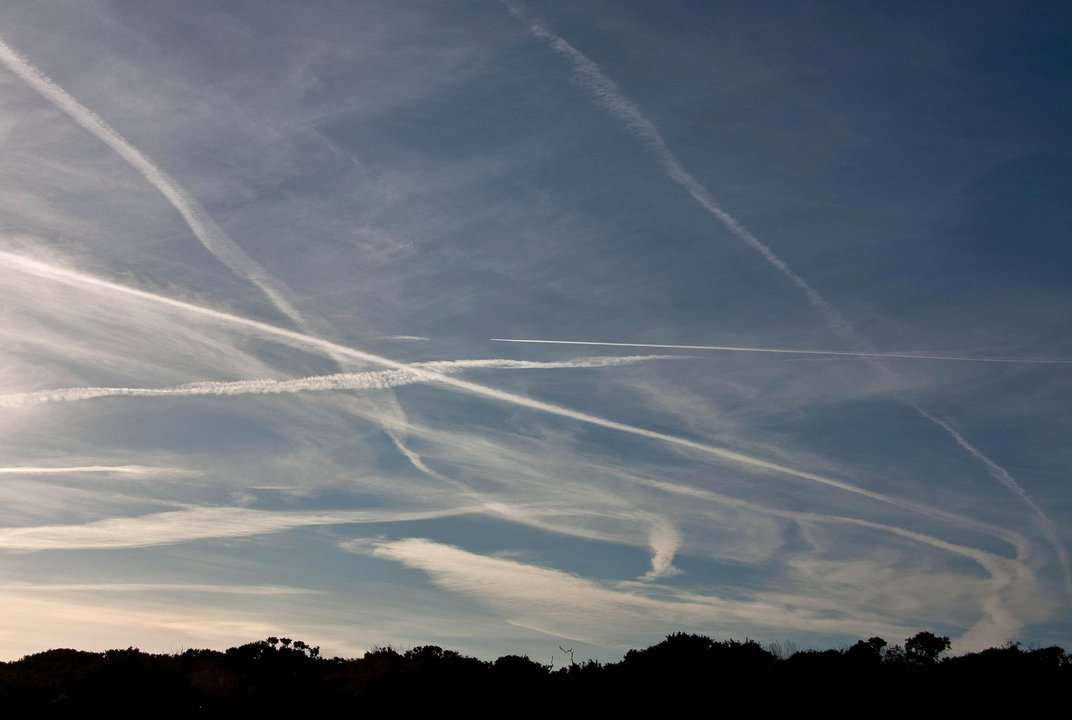
\includegraphics[width=5cm]{10836877206_1f0c305cce_k.jpg}}
\column{.5\textwidth}\vbox to \textheight{
\centering
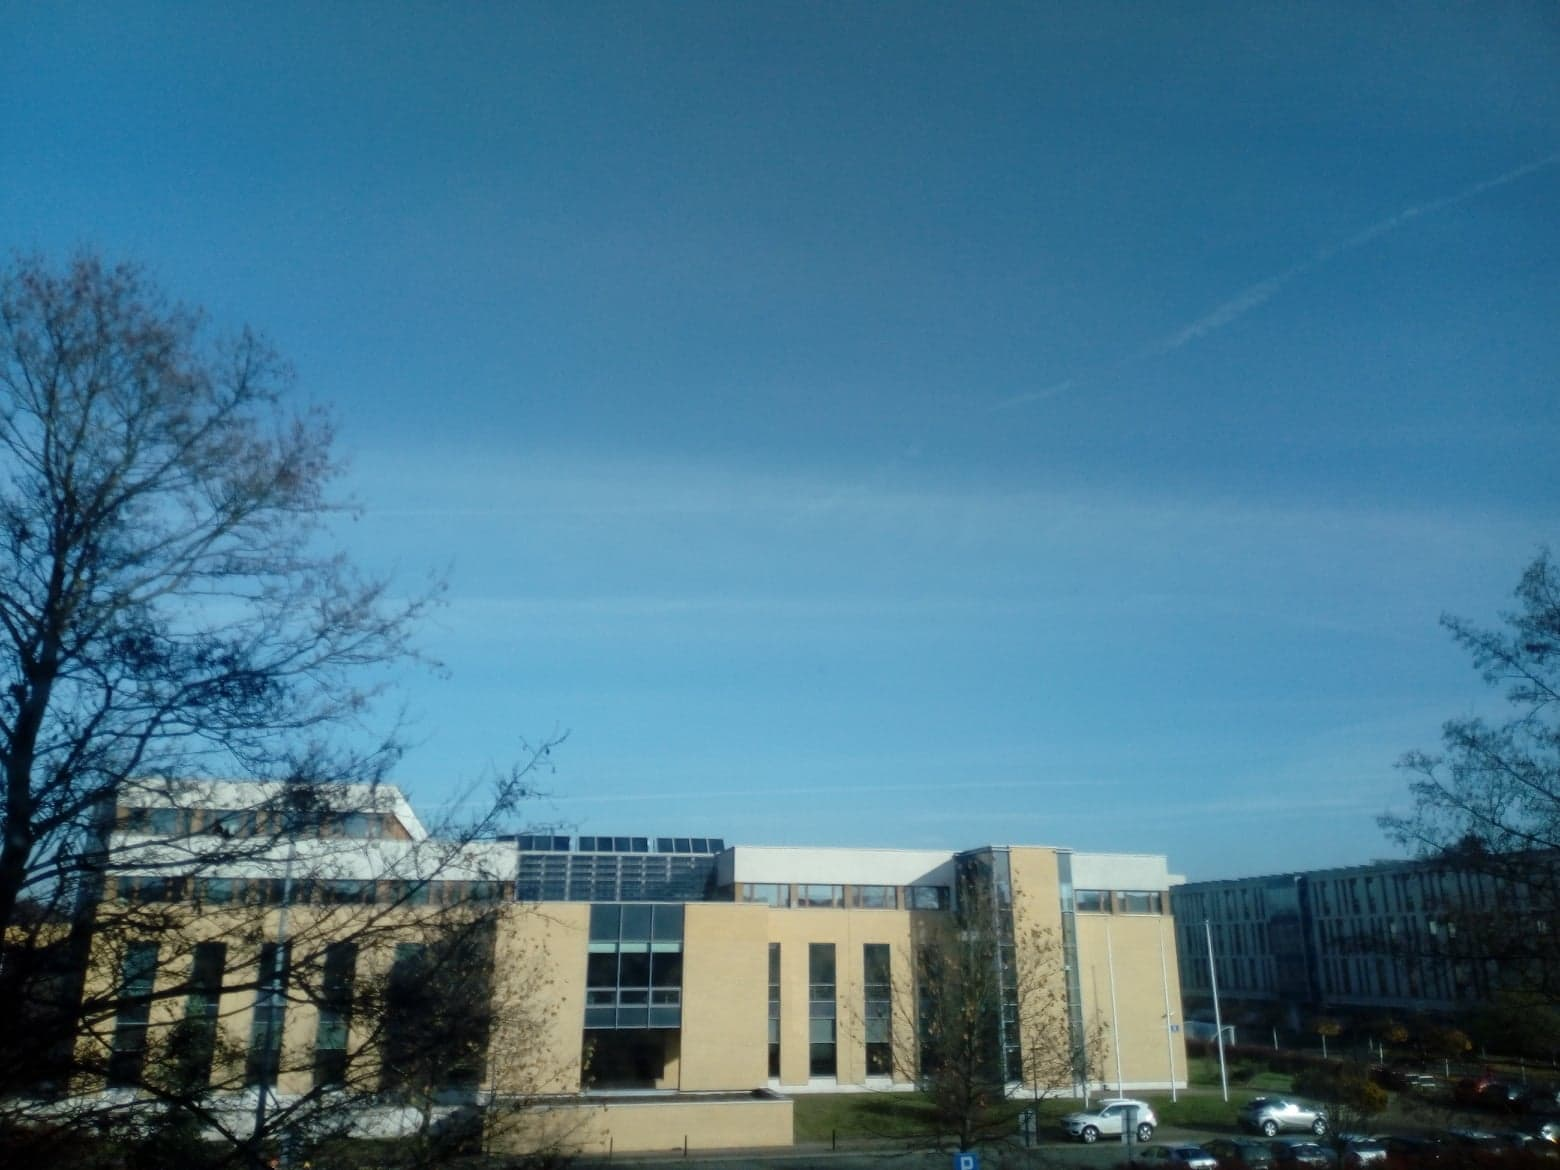
\includegraphics[width=5cm]{316451350_546801620641032_8394163998293391517_n.jpg}\\ \vfill
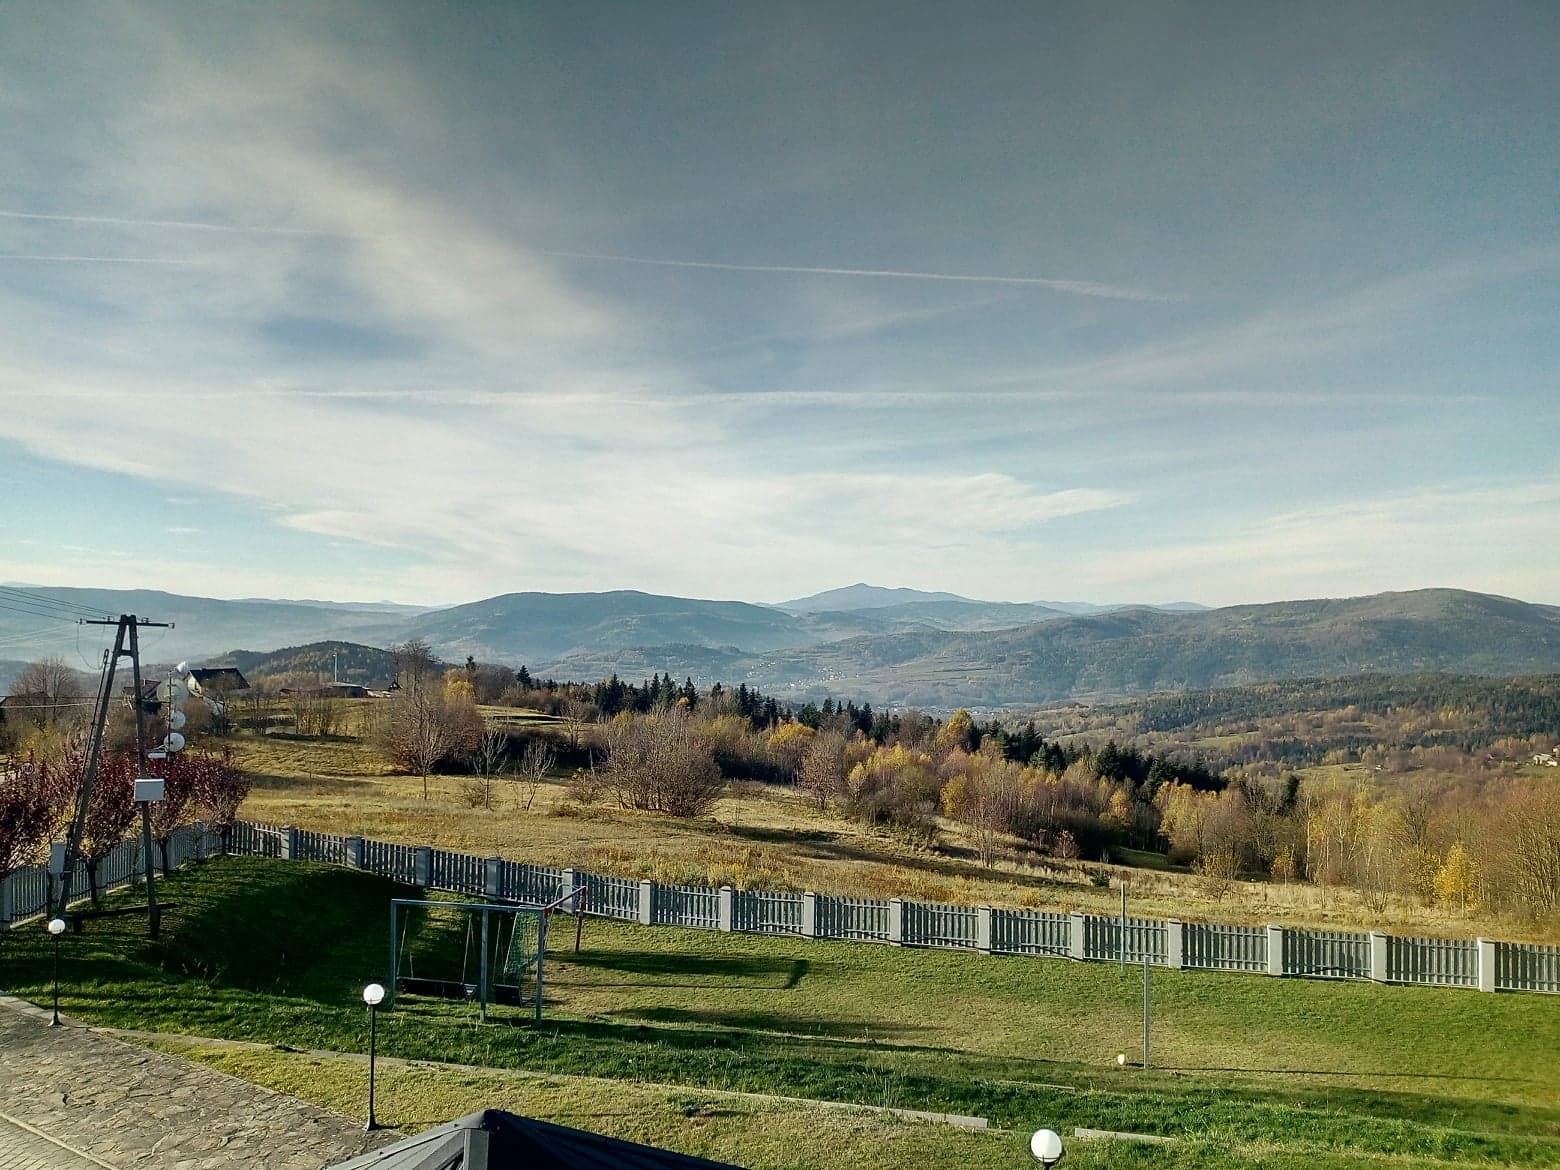
\includegraphics[width=5cm]{316778754_619311233324597_5501881348319323448_n.jpg}}
\end{columns}
\end{frame}

\begin{frame}{Contrails and chemtrails}
   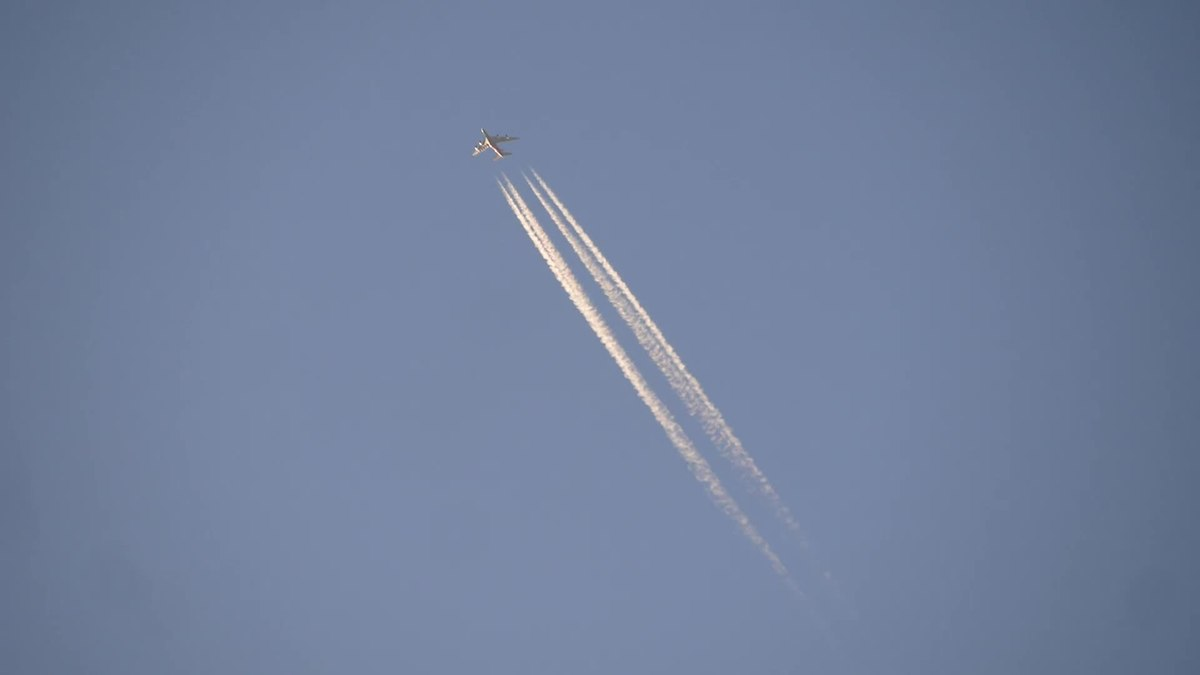
\includegraphics[align=c,width=5cm]{1200px--Jet-contrails-tokyosky-japan-2018.webm.jpg}\hfill
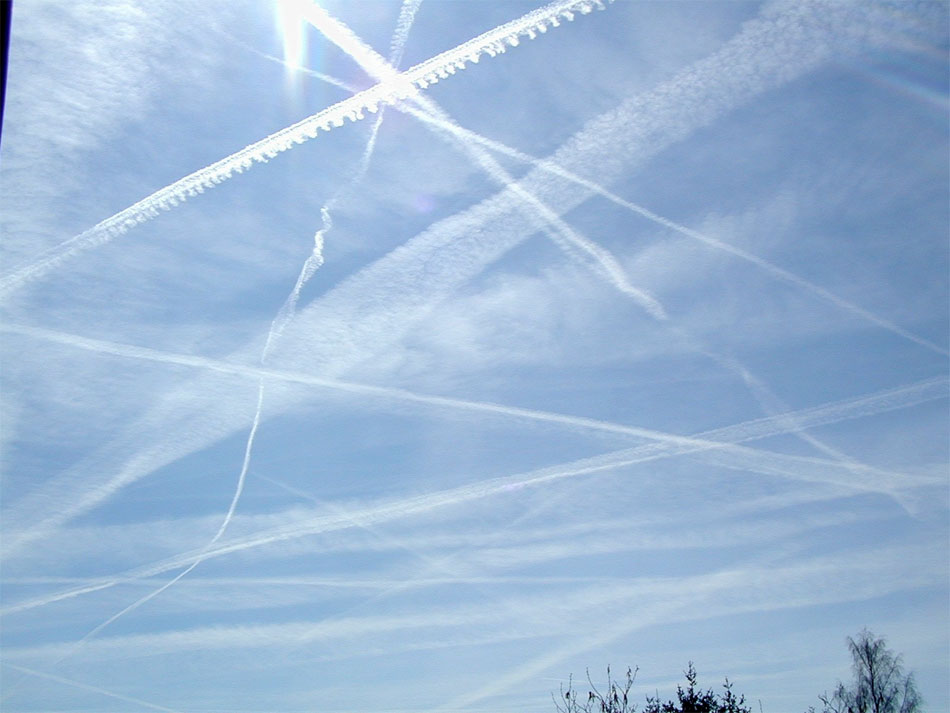
\includegraphics[align=c,width=5cm]{chemtrails.jpg}
\end{frame}

\begin{frame}{History}

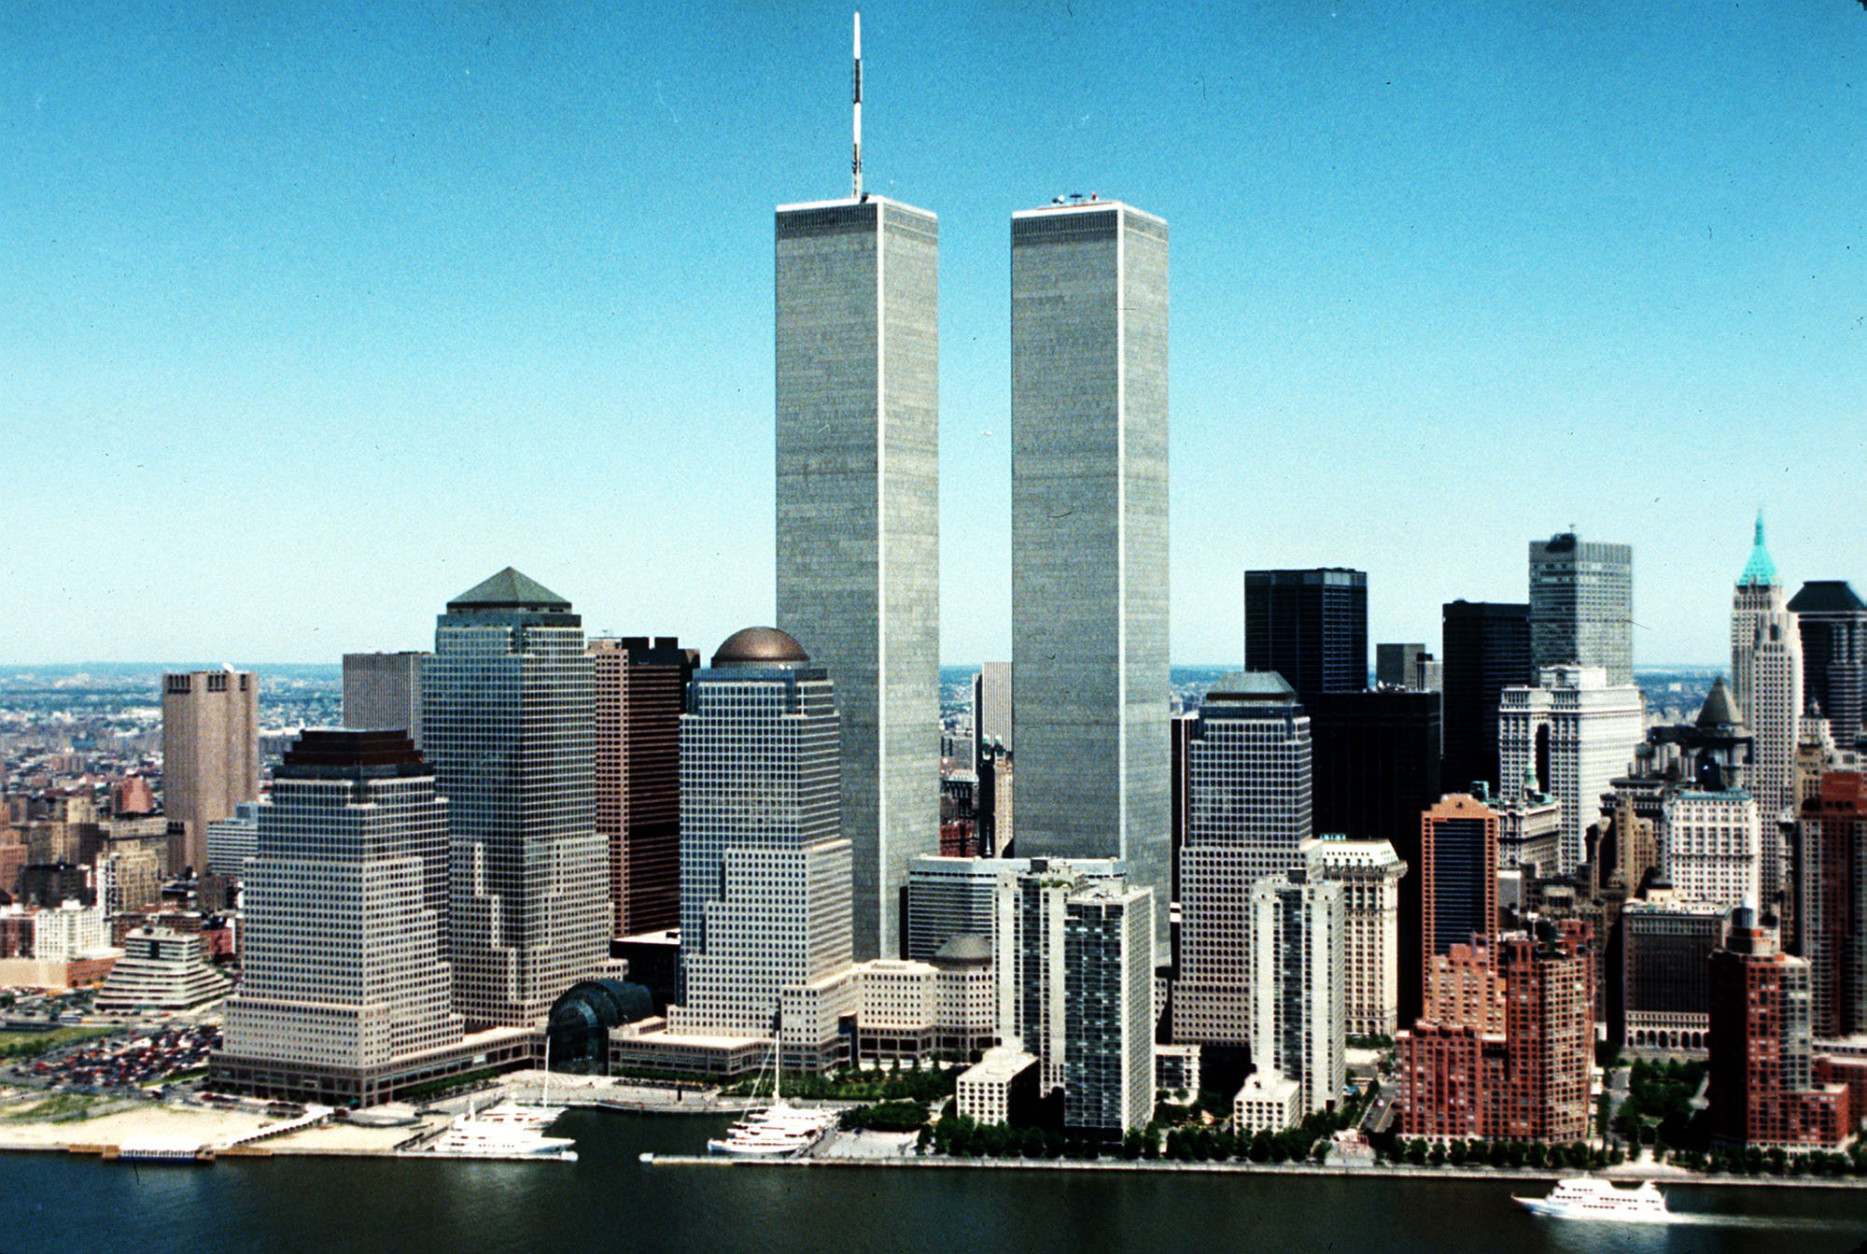
\includegraphics[align=c,width=5cm]{AP_90010117493-1867x1254.jpg}\hfill
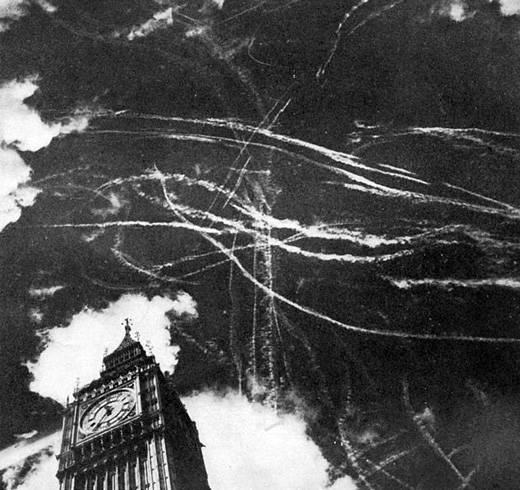
\includegraphics[align=c,width=5cm]{sZBO3IR.jpg}
    
\end{frame}



%\section{Założenia}

\begin{frame}{Spraying mechanism}


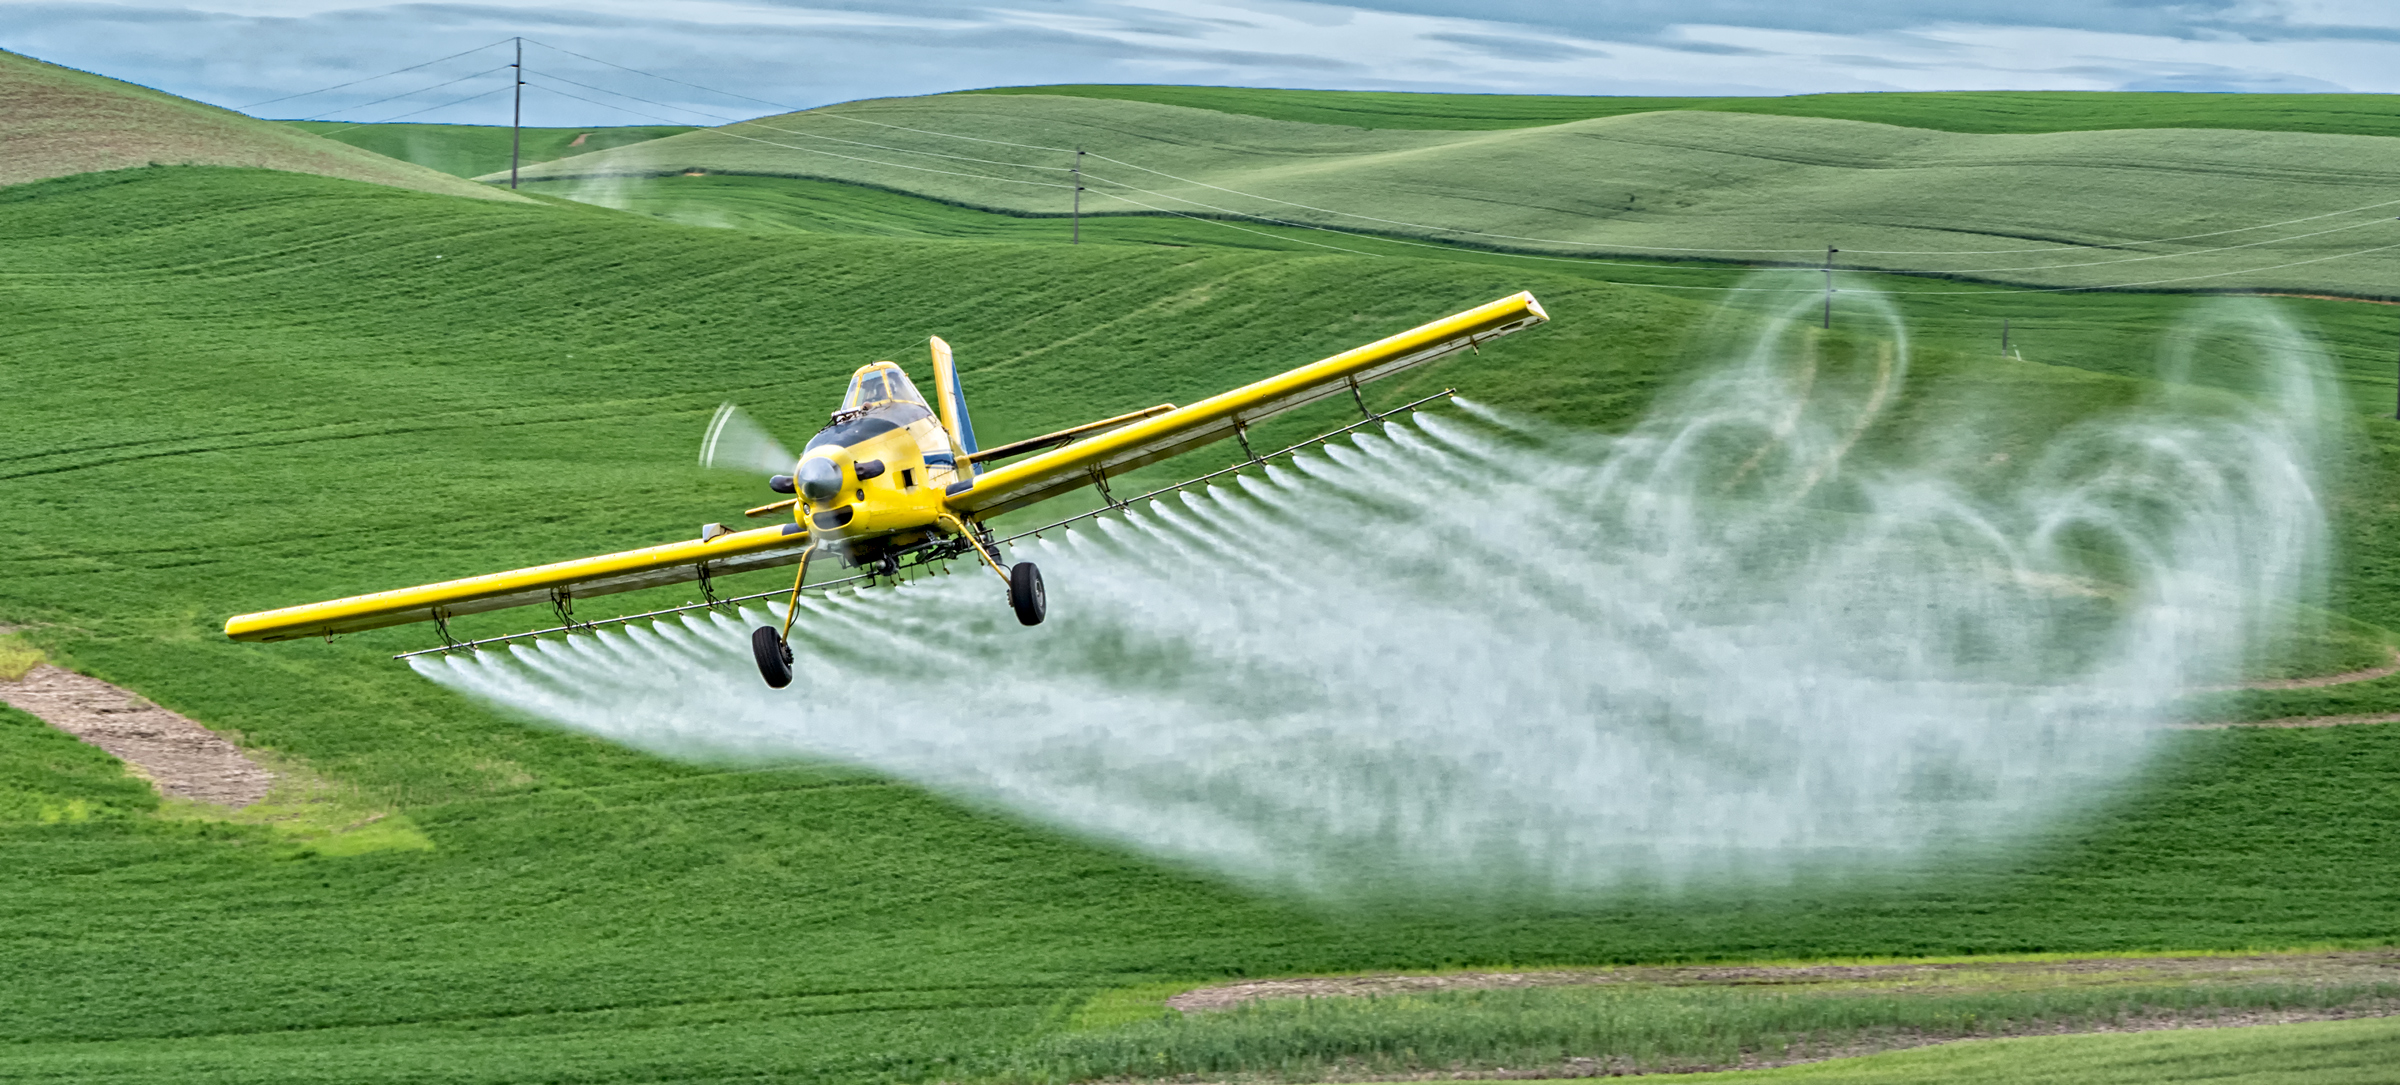
\includegraphics[align=c,width=5cm]{Crop-Duster-2.jpg}\hfill
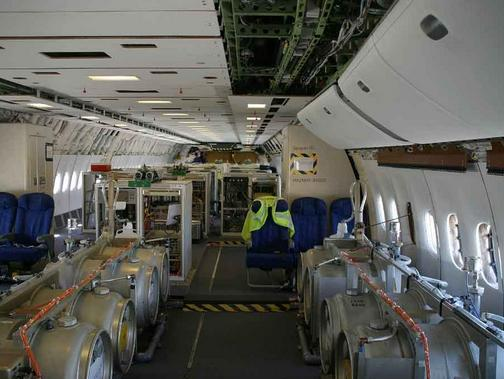
\includegraphics[align=c,width=5cm]{gdfhthrtjjrj.JPG}



\end{frame}

\begin{frame}{Not only engines}


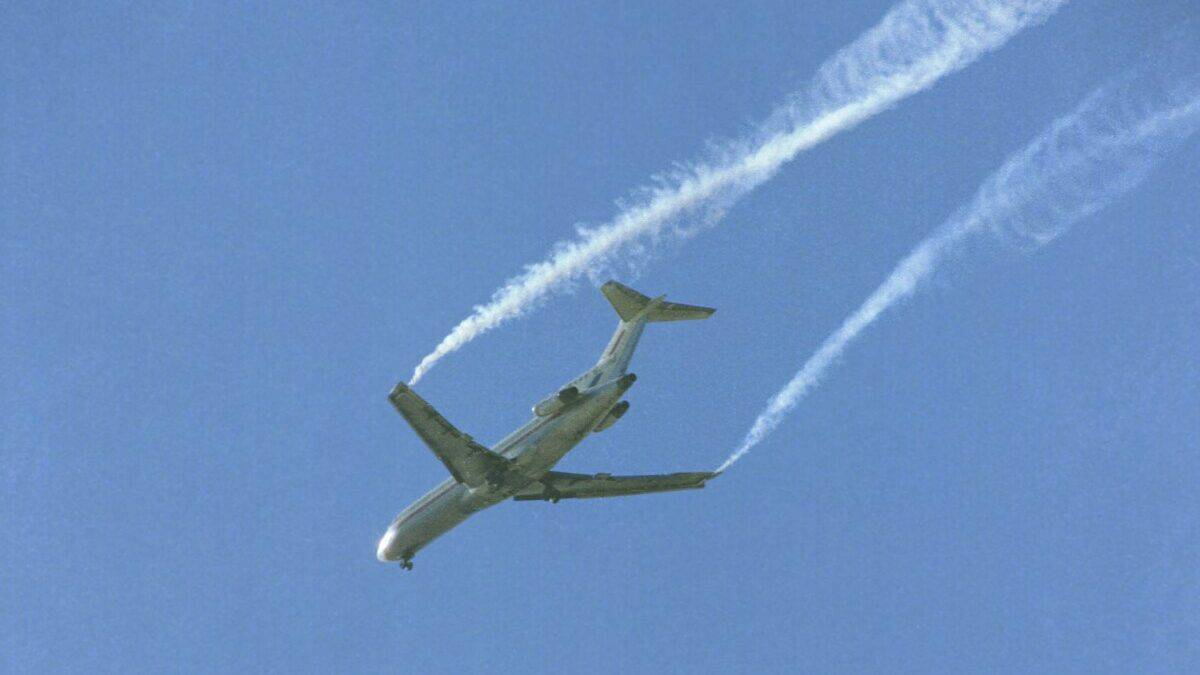
\includegraphics[align=c,width=5cm]{Airplane-Vortices-edited.jpg}\hfill
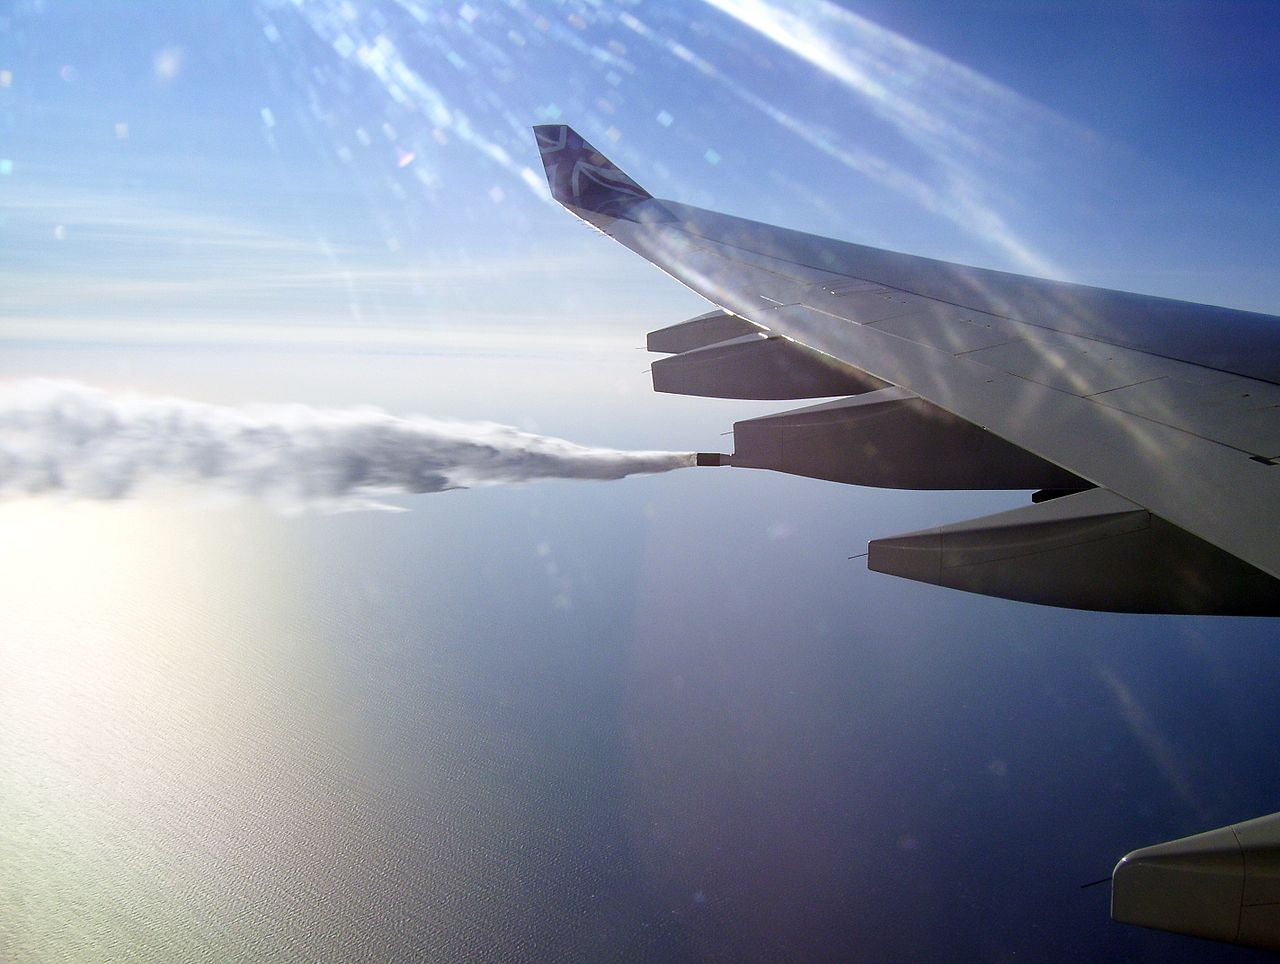
\includegraphics[align=c,width=5cm]{1280px-FuelDumpA340-600.JPG}



\end{frame}

\section[Part II. Realisation]{Part II\\Realisation: Chemtrails do not exist}



\begin{frame}
\begin{columns}[t]
\column{.5\textwidth}\vbox to \textheight{
\centering
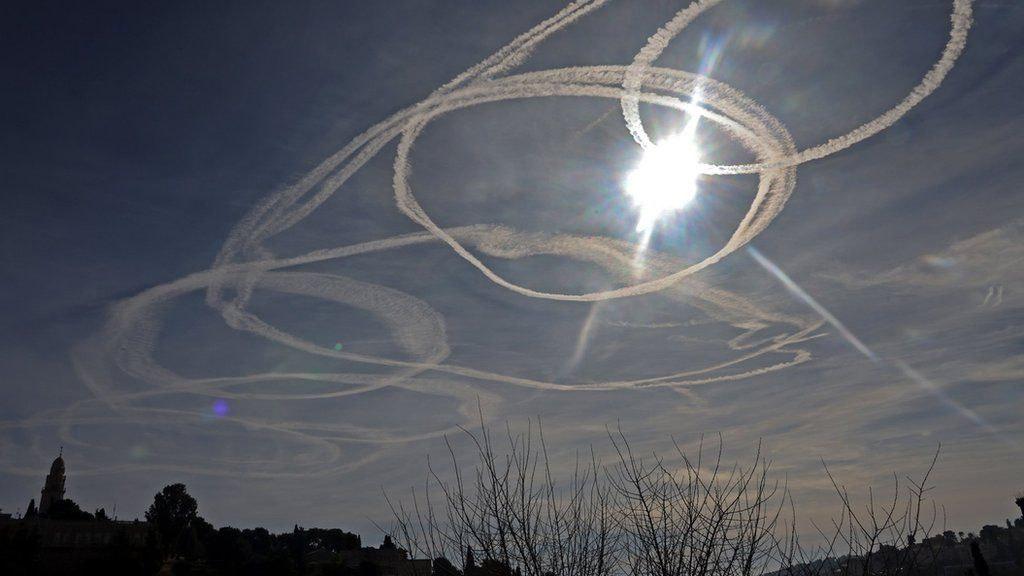
\includegraphics[width=5cm]{_126014953_gettyimages-1230798088.jpg} \\ \vfill
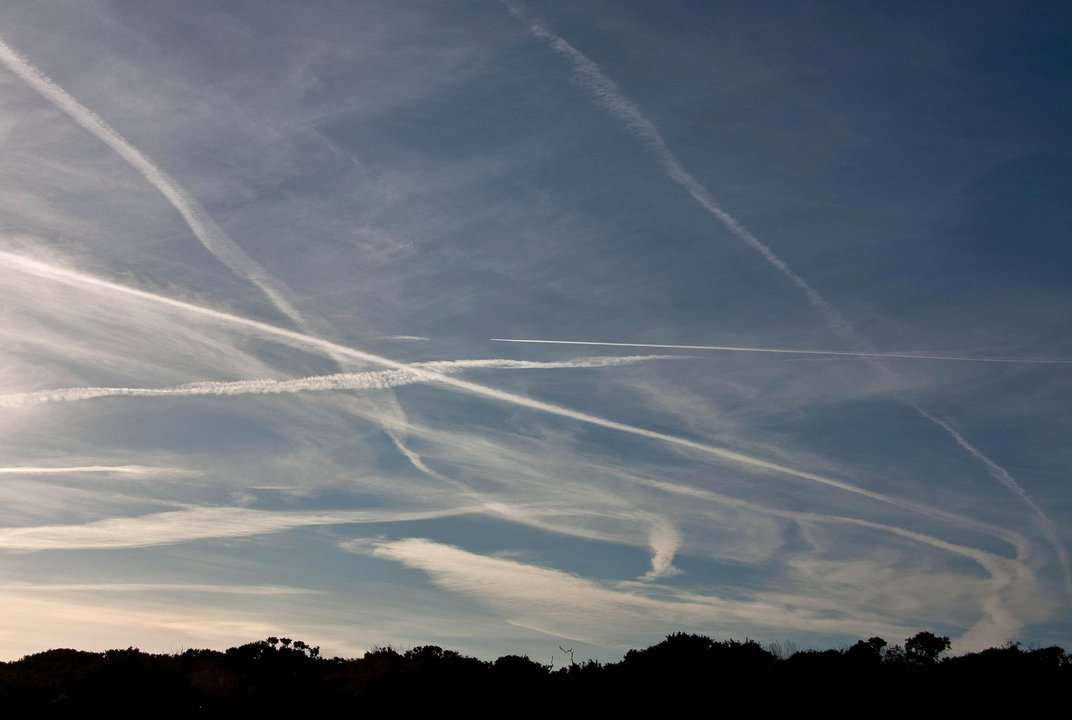
\includegraphics[width=5cm]{10836877206_1f0c305cce_k.jpg}}
\column{.5\textwidth}\vbox to \textheight{
\centering
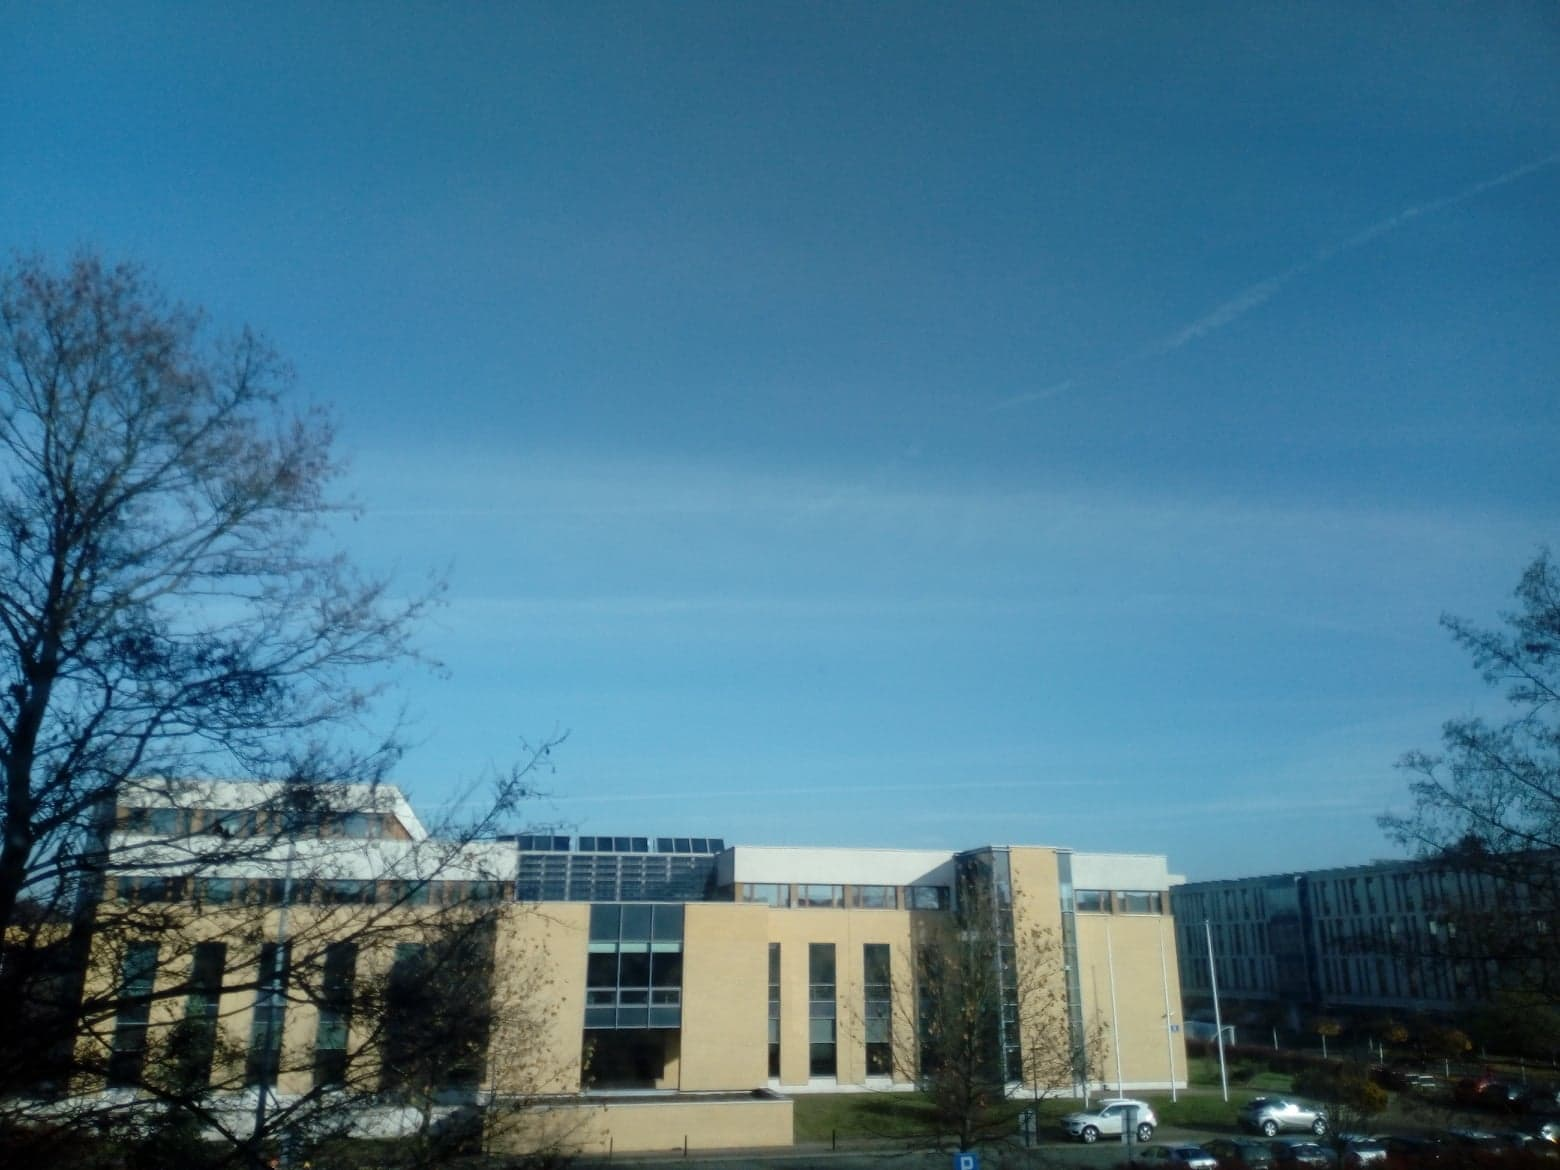
\includegraphics[width=5cm]{316451350_546801620641032_8394163998293391517_n.jpg}\\ \vfill
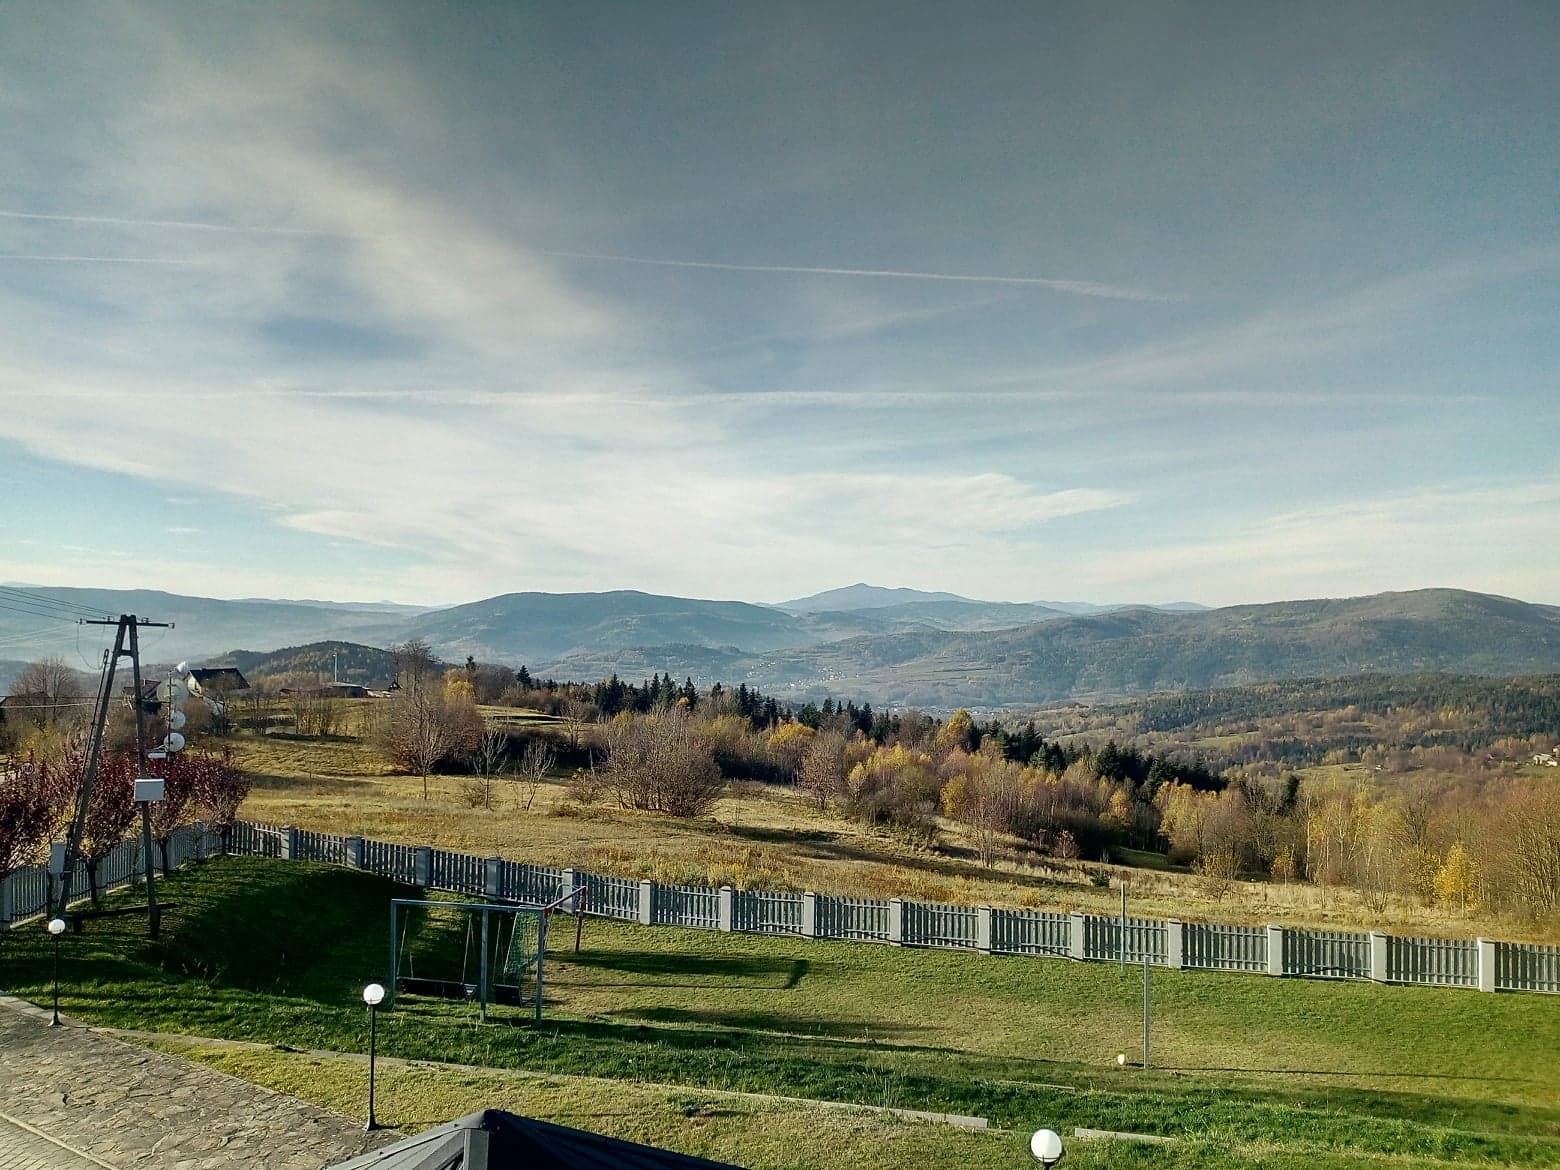
\includegraphics[width=5cm]{316778754_619311233324597_5501881348319323448_n.jpg}}
\end{columns}
\end{frame}

\begin{frame}{Contrails and chemtrails}
   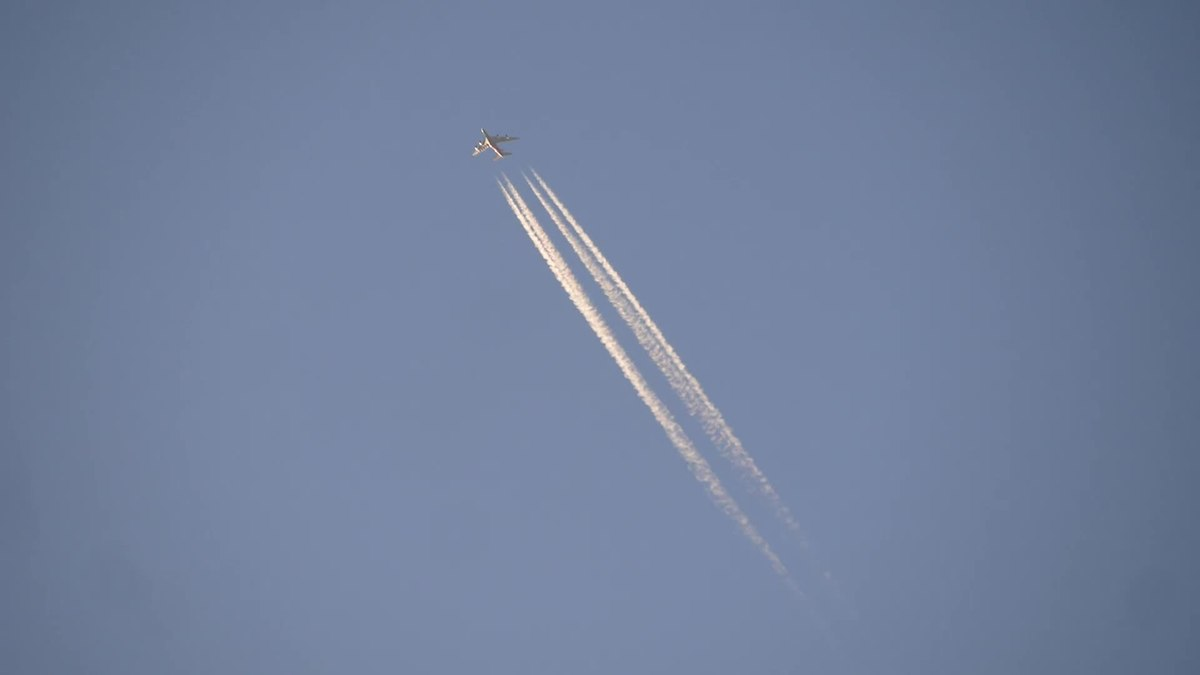
\includegraphics[align=c,width=5cm]{1200px--Jet-contrails-tokyosky-japan-2018.webm.jpg}\hfill
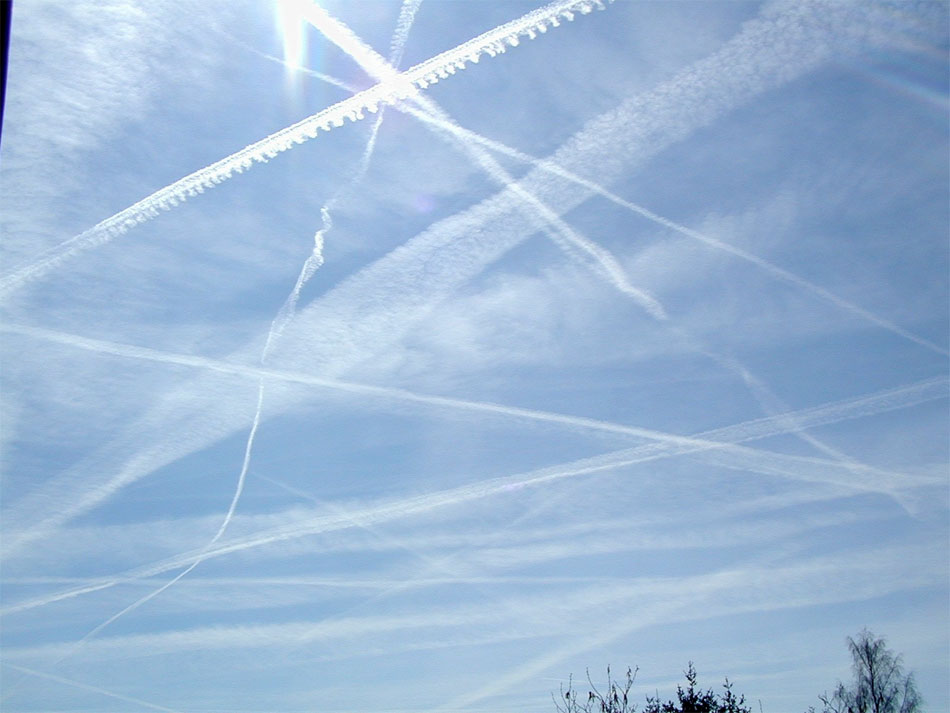
\includegraphics[align=c,width=5cm]{chemtrails.jpg}
\end{frame}

\begin{frame}{History}

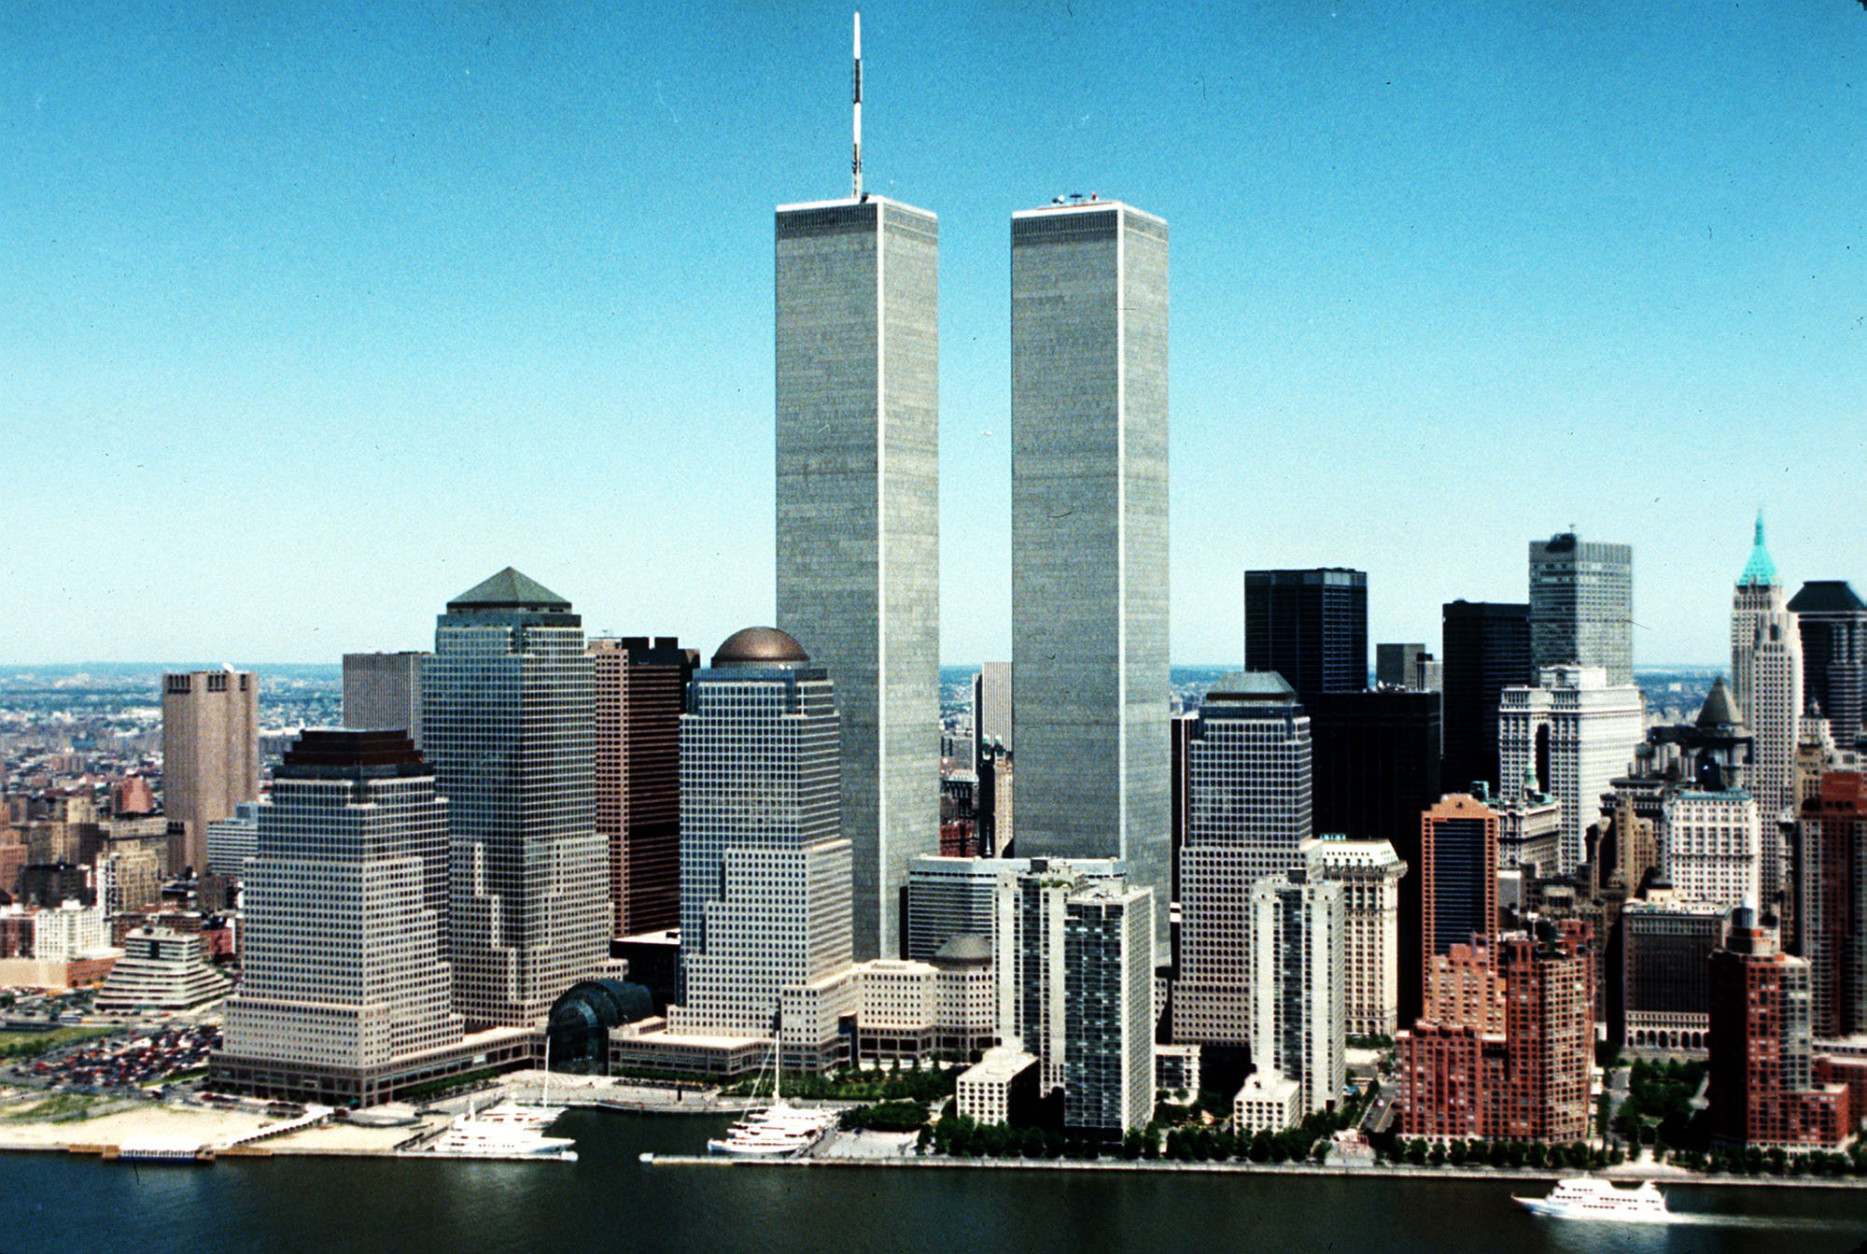
\includegraphics[align=c,width=5cm]{AP_90010117493-1867x1254.jpg}\hfill
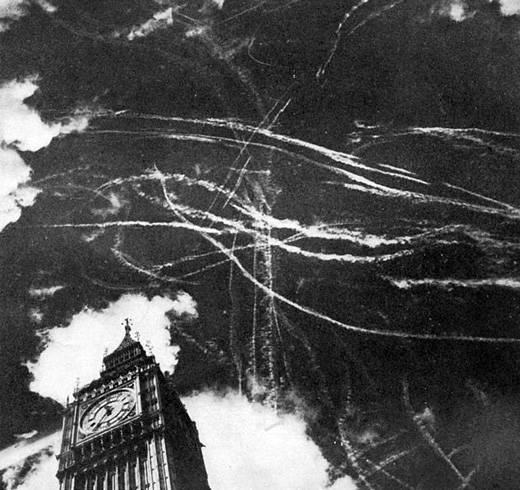
\includegraphics[align=c,width=5cm]{sZBO3IR.jpg}
    
\end{frame}



%\section{Założenia}

\begin{frame}{Spraying mechanism}


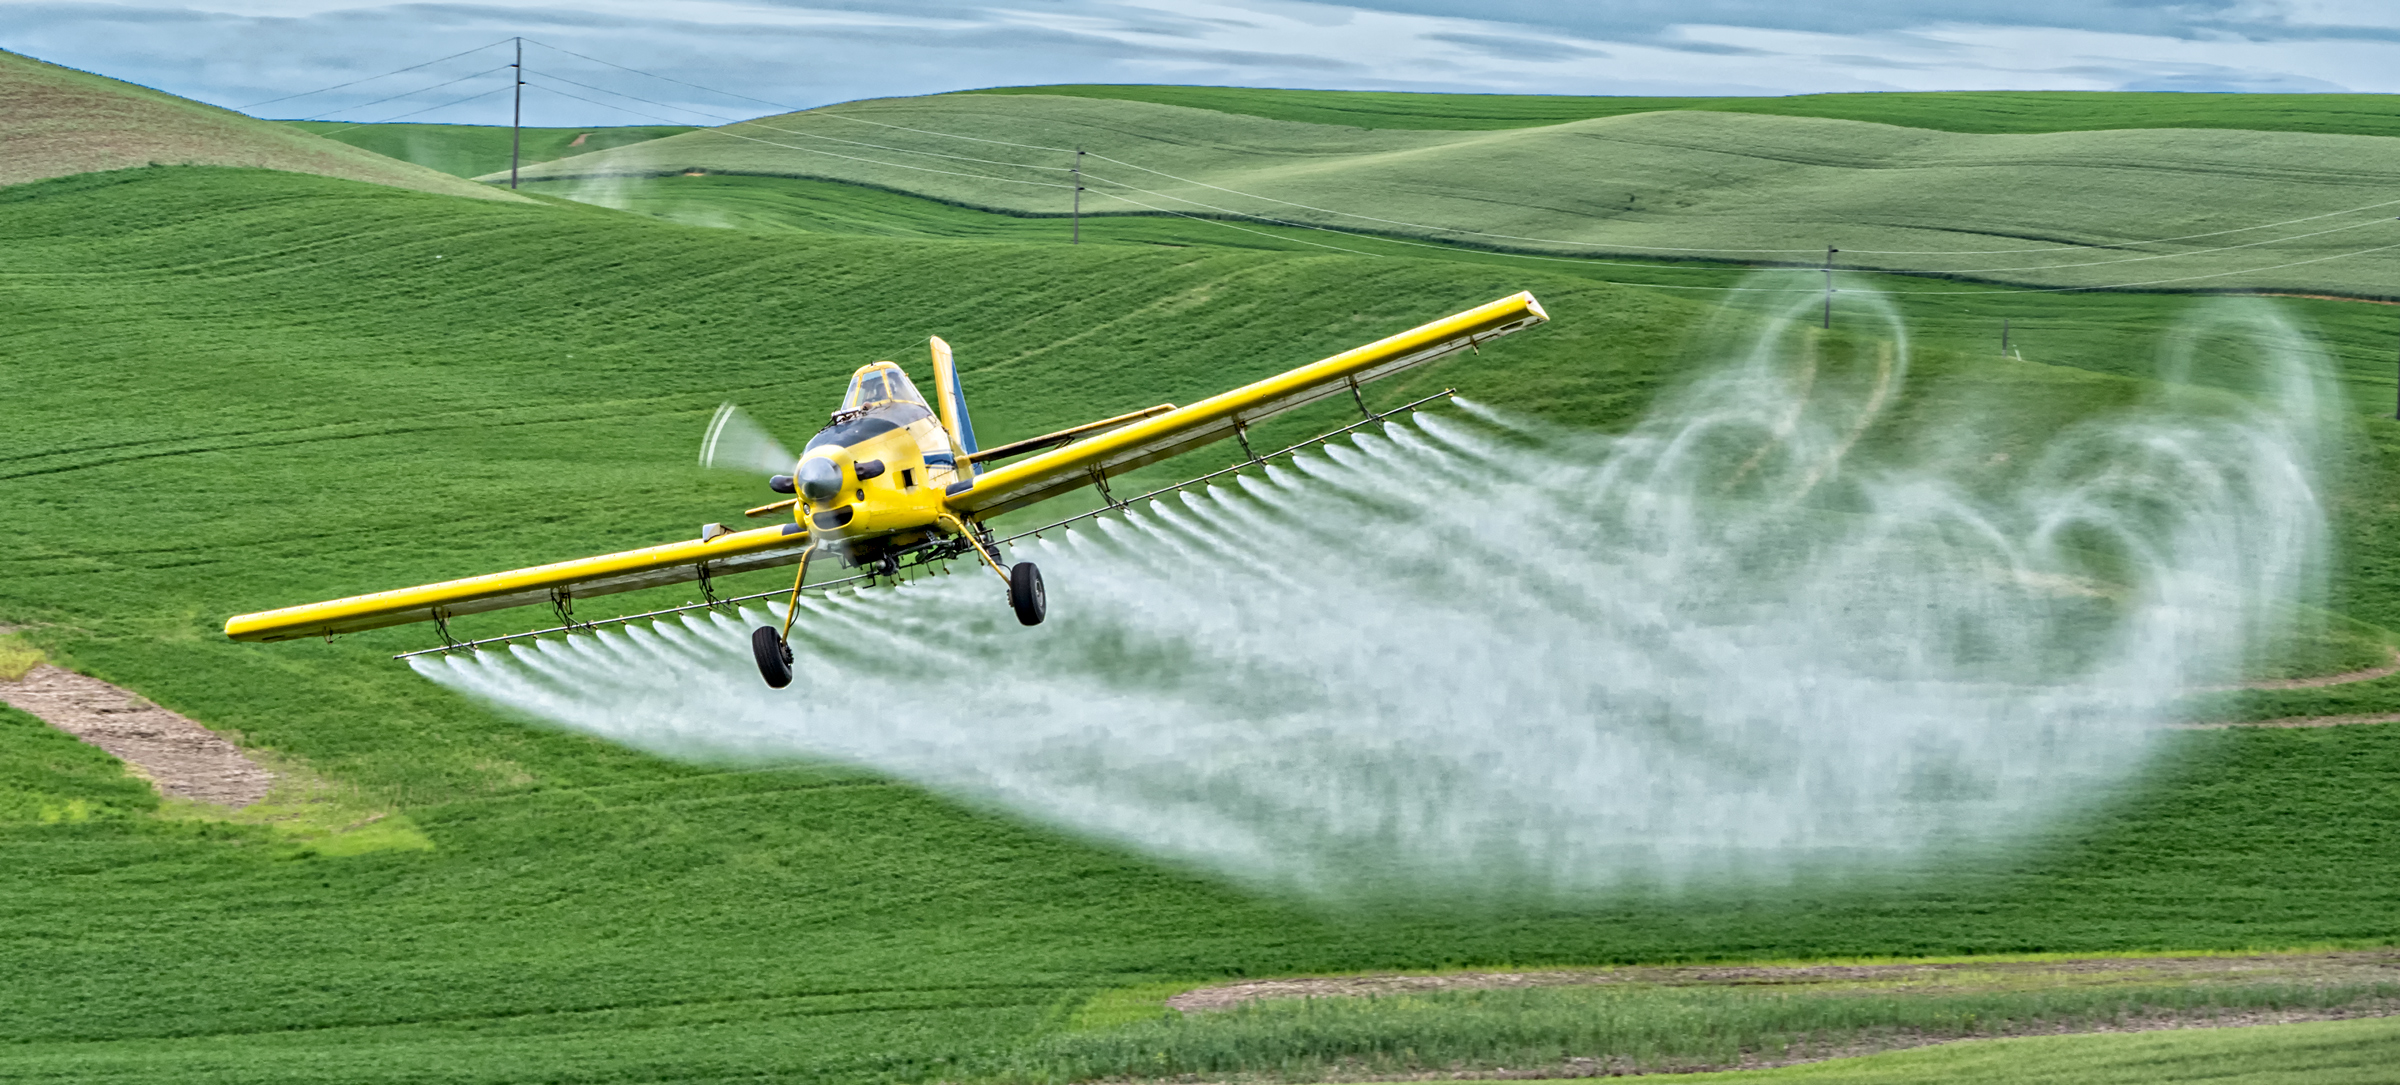
\includegraphics[align=c,width=5cm]{Crop-Duster-2.jpg}\hfill
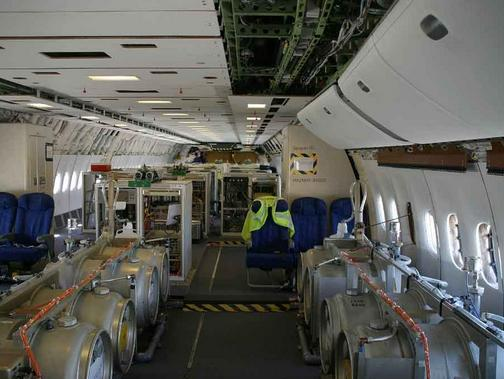
\includegraphics[align=c,width=5cm]{gdfhthrtjjrj.JPG}



\end{frame}

\begin{frame}{Not only engines}


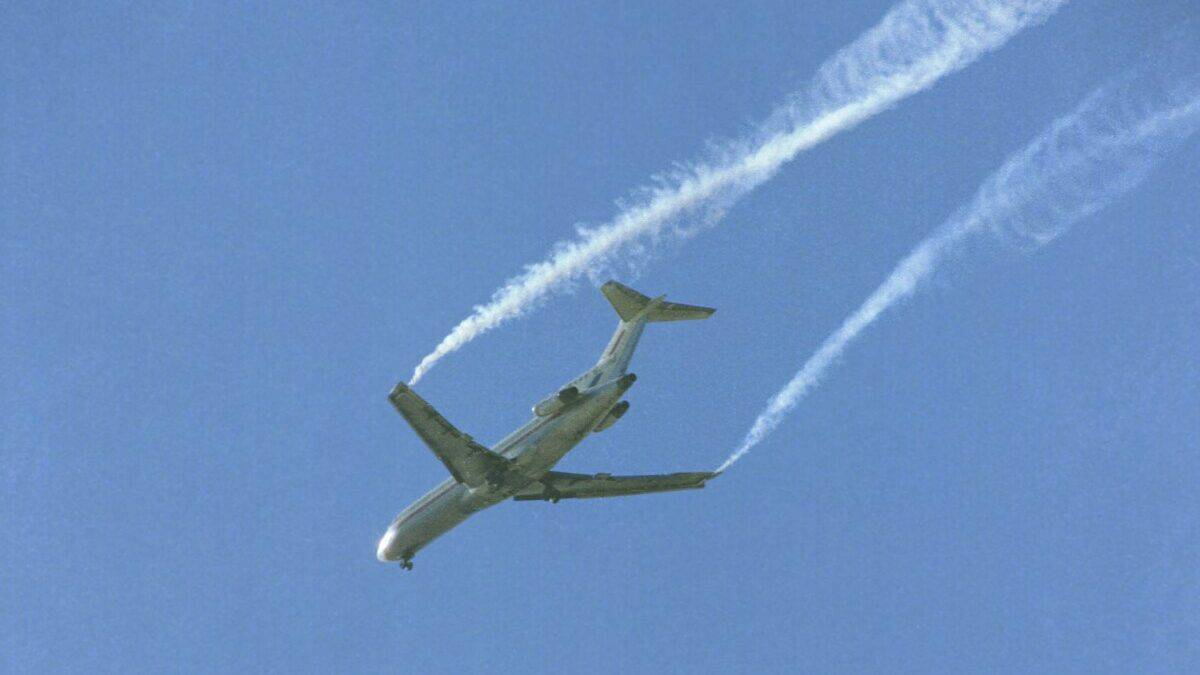
\includegraphics[align=c,width=5cm]{Airplane-Vortices-edited.jpg}\hfill
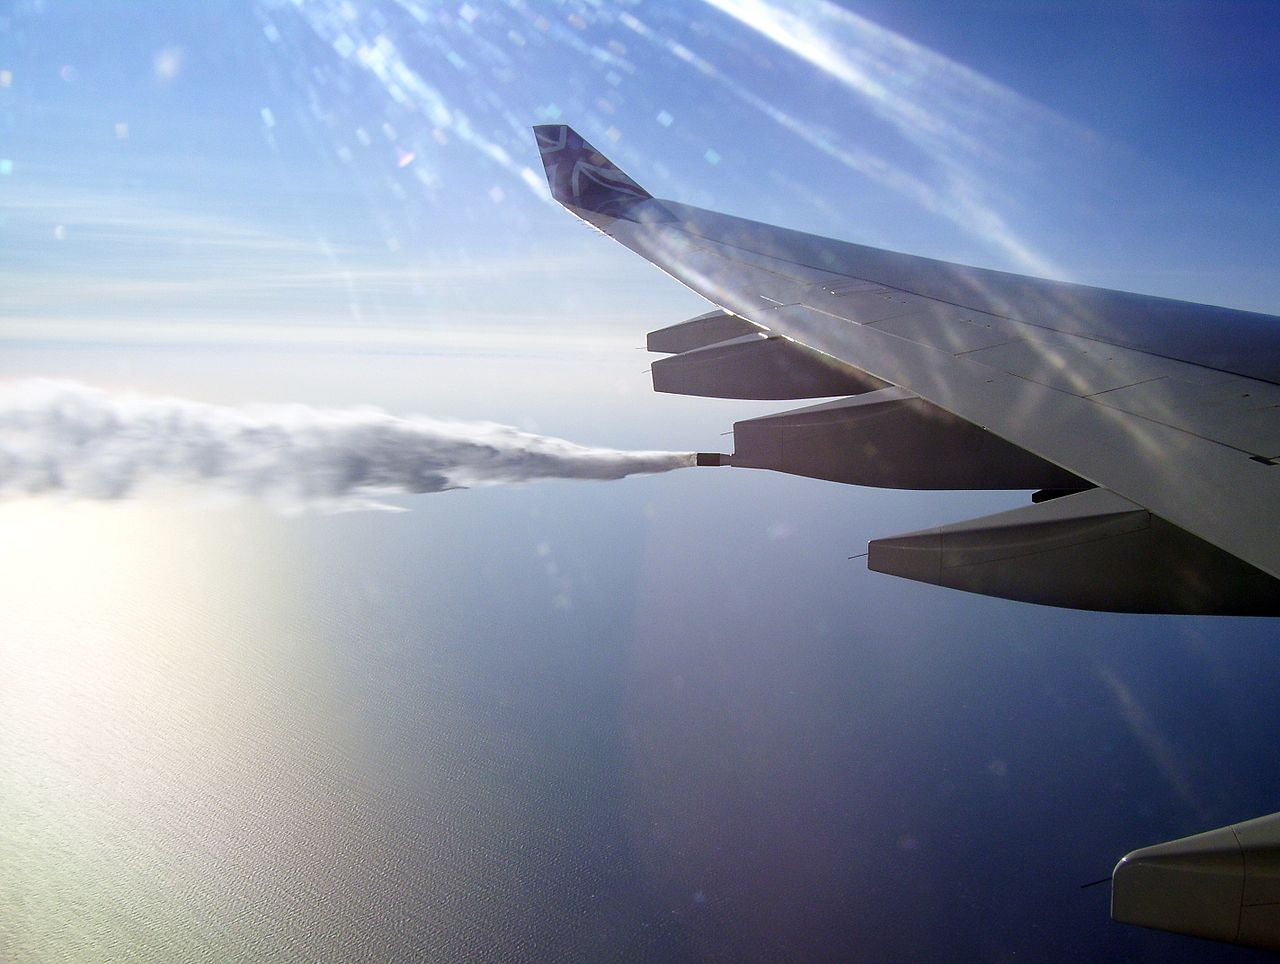
\includegraphics[align=c,width=5cm]{1280px-FuelDumpA340-600.JPG}



\end{frame}

\begin{frame}\vfill
    

\begin{figure}
\centering
    \begin{tikzpicture}
      \duck[parrot, body=gray!30!white, head=gray!30!white, bill=red, water=cyan!50!blue, magichat, scale=1.2]
      \fill[cyan!20!white] (-1.9,1.8) ellipse (2.2 and 0.5);
  \fill[cyan!20!white] (-0.2,1.54) -- (0.2,1.35) -- (0.0,1.6) -- cycle;
	\node at (-1.9,1.8) {Thanks for your attention};
    \end{tikzpicture}
    \end{figure}
    
    \vfill
\end{frame}



\end{document}